\documentclass[oneside]{book}

\usepackage[english]{babel}
\usepackage[T1]{fontenc} 
\usepackage[utf8]{inputenc}
\usepackage{amsmath}
\usepackage{amssymb}
\usepackage{amsfonts}
\usepackage{graphicx}
\usepackage[ruled]{algorithm2e}
\usepackage{empheq}
\usepackage{float}
\usepackage{listings}
\usepackage{color}

\definecolor{dkgreen}{rgb}{0,0.6,0}
\definecolor{gray}{rgb}{0.5,0.5,0.5}
\definecolor{mauve}{rgb}{0.58,0,0.82}
\definecolor{blck}{rgb}{0,0,0}

\lstset{frame=tb,
  language=Java,
  keepspaces=true,
  aboveskip=3mm,
  belowskip=3mm,
  showstringspaces=false,
  columns=flexible,
  basicstyle={\small\ttfamily},
  numbers=none,
  numberstyle=\tiny\color{gray},
  keywordstyle=\color{blue},
  commentstyle=\color{dkgreen},
  stringstyle=\color{mauve},
  breaklines=true,
  breakatwhitespace=true
  tabsize=3
}

\title{Algorithmic Programming in Java}
\author{Rodion Efremov} 
\date{}

\begin{document}
\maketitle

\chapter*{Preface}
This book is aiming to provide insight into practical implementation of algorithms and data structures in a way that is as accessible to readers of all proficiency levels. Only very basic knowledge of Java programming language and other tools is assumed; wherever relevant, the new language features are explained succinctly without further ado. The book is organized in a ``bottom-up'' fashion so that the book is better read linearly, but not necessarily continuously whenever some topics do not interest. There is no exercises. Instead, the book presents the code listings for a Java library of algorithms and data structures, so the book might be used as a collection of ``algorithmic recipes''. 

The second objective is to provide a gentle introduction to formalism taking place in computer science independent of particular tool sets. By formalism we mean most often pseudo-code, big O notation, set notation, sequences and functions. We, however, will not do any fancy mathematics with Greek letters such as proving theorems, etc. Whether to learn formalism or not mainly depends on your academic aims: in case you are planning to enroll in a department of computer science, this book just might be everything you need to get prepared for your studies.

\makeatletter\@openrightfalse
\part{Introduction}
This part will introduce the reader to common ground for successive parts of the book. The topics covered are coding conventions for the library we will implement, using \textbf{Maven} to manage your version of the library, and using \textbf{git} to store your version of the library.

\chapter{Coding conventions}
\@openrighttrue\makeatother
\section{Naming types, methods and variables}
The Java community encourages using ``CameCase'' to name your identifiers. For instance, \texttt{elementAmount}, \texttt{nodePriority} are identifiers for local variables or class fields adhering to CamelCase style. Following the intuition, \texttt{getSize} or \texttt{decreasePriority} are (in some sense) ``good'' names for class methods. The naming convention for user-defined types makes a small exception to the above rule: the first letter is capitalized: \texttt{PathFinder}, \texttt{DirectedGraphNode}.

\section{Fluent API}
While developing a software library $L$, the top priority is keeping $L$'s API (application programming interface) as simple as possible. Simplicity does not come automatically with the presence of Javadoc\footnote{A documenting tool included in Java Development Kit.} for each class in $L$. Consider the following code snippet:
\begin{lstlisting}
Node source = ...;
Node target = ...;
Path<Node> p = new DijkstraFinder<Node>().search(source, target);
\end{lstlisting}
\newpage
\noindent This is intuitive and easy to remember. On the contrary, the following is not quite:
\begin{lstlisting}[caption={Too much arguments for a method call},label=lst:bidirastarfinder1]
Node source = ...;
Node target = ...;
PriorityQueue<Node> queue = ...;
HeuristicFunction<Node> h1 = ...;
HeuristicFunction<Node> h2 = ...;
Path<Node> p = new BidirectionalAStarFinder<Node>().search(source, 
							   target, 
							   queue, 
							   h1, 
							   h2);
\end{lstlisting}
There is a way to make an API more convenient, and it is usually called ``fluent'' API, where a call to a function is prepared argument by argument in the following manner:
\begin{lstlisting}
Path<Node> p = usingBidirectionalAStarFinder<Node>
              .from(source)
              .to(target)
              .withPriorityQueue(queue)
              .withForwardHeuristic(h1)
              .withBackwardsHeuristic(h2)
              .search();
\end{lstlisting}
The above listing is an improvement over Listing \ref{lst:bidirastarfinder1}.
Now that we know the name of the technique, let's see a working example:
\lstset{
  numbers=left
}
\begin{lstlisting}
public class Main {
    
    public static void main(String... args) {
        String result1 = begin().withSource("France")
                                .withTarget("Japan")
                                .withAlgorithm1();
        
        String result2 = begin().withSource("Germany")
                                .withTarget("Finland")
                                .withAlgorithm2();
        
        System.out.println(result1);
        System.out.println(result2);
    }
    
    static SourceNodeSelector begin() {
        return new SourceNodeSelector();
    }
}

abstract class Algorithm {
    protected TargetNodeSelector targetNodeSelector;
    
    abstract String execute();
    
    Algorithm(TargetNodeSelector targetNodeSelector) {
        this.targetNodeSelector = targetNodeSelector;
    }
}

class Algorithm1 extends Algorithm {
    
    Algorithm1(TargetNodeSelector targetNodeSelector) {
        super(targetNodeSelector);
    }
    
    String execute() {
        return "ALGORITHM1 from " + targetNodeSelector.getSource() + " to " +
               targetNodeSelector.getTarget();
    }
}

class Algorithm2 extends Algorithm {
    
    Algorithm2(TargetNodeSelector targetNodeSelector) {
        super(targetNodeSelector);
    }
    
    String execute() {
        return "ALGORITHM2 from " + targetNodeSelector.getSource() + " to " +
                targetNodeSelector.getTarget();
    }
}

class SourceNodeSelector {
    private String source;
    
    TargetNodeSelector withSource(String source) {
        this.source = source;
        return new TargetNodeSelector(this);
    }
    
    String getSource() {
        return source;
    }
}

class TargetNodeSelector {
    private SourceNodeSelector sourceNodeSelector;
    private String target;
    
    TargetNodeSelector(SourceNodeSelector sourceNodeSelector) {
        this.sourceNodeSelector = sourceNodeSelector;
    }
    
    AlgorithmSelector withTarget(String target) {
        this.target = target;
        return new AlgorithmSelector(this);
    }
    
    SourceNodeSelector getSourceNodeSelector() {
        return sourceNodeSelector;
    }
    
    String getSource() {
        return sourceNodeSelector.getSource();
    }
    
    String getTarget() {
        return target;
    }
}

class AlgorithmSelector {
    private TargetNodeSelector targetNodeSelector;
    
    AlgorithmSelector(TargetNodeSelector targetNodeSelector) {
        this.targetNodeSelector = targetNodeSelector;
    } 
    
    public String withAlgorithm1() {
        return new Algorithm1(targetNodeSelector).execute();
    }
    
    public String withAlgorithm2() {
        return new Algorithm2(targetNodeSelector).execute();
    }
}
\end{lstlisting}
You can see a fluent API in action at lines 4 and 8. First of all, this is more explicit about the meaning of each argument passed to a method. Second point is the fact that the sequence of arguments being ``built'' is fixed, you cannot write \texttt{withTarget(...)} before \texttt{withSource(...)}. Also, you will get a compilation error whenever you forget to specify an argument of a fluent API call:
\newpage
\lstset{
numbers=none
}
\begin{lstlisting}[caption={Bad fluent API call},label=lst:badfluentapi]
begin().withSource("France")
       .withAlgorithm1();  // Compile-time error: withSource returns 
                           // TargetNodeSelector which has no 
                           // withAlgorithm1.
\end{lstlisting}
The last but not least, modern IDE's (integrated development environments) support code-completion, which makes it easier to write syntactically correct code. For instance, in Listing \ref{lst:badfluentapi}, a good IDE, after writing \\ \texttt{begin().withSource(...)}, will give a list of suggestions containing \texttt{withTarget} - method. That way, you don't need to remember each and every function, the IDE will guide you through making calls to a fluent API methods.

\section{Using Maven for managing the projects}
Developing a library regardless of a language, usually results in dozens of files, which makes it inconvenient to work at the lowest level (invoking \textbf{javac} and \textbf{java} every time she or he recompiles a project). Maven is a build tool remedying the issue. First, we might want to create Maven-driven Java project:
\begin{verbatim}
mvn archetype:create -DgroupId=com.example -DartifactId=my-proj
\end{verbatim}
The above spell will take the current working directory and create in it a following file system tree:
\begin{center}
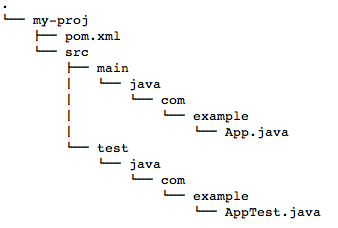
\includegraphics[width=240px,keepaspectratio]{mvntree}
\end{center}
If you look at it, you may guess that the file \textbf{pom.xml} configures the project we just created:
\lstset{
language=XML,
keywordstyle=\color{blck},
}
\begin{lstlisting}
<project xmlns="http://maven.apache.org/POM/4.0.0"
         xmlns:xsi="http://www.w3.org/2001/XMLSchema-instance"
         xsi:schemaLocation="http://maven.apache.org/POM/4.0.0
         http://maven.apache.org/xsd/maven-4.0.0.xsd">
  <modelVersion>4.0.0</modelVersion>

  <groupId>com.example</groupId>
  <artifactId>my-proj</artifactId>
  <version>1.0-SNAPSHOT</version>
  <packaging>jar</packaging>

  <name>my-proj</name>
  <url>http://maven.apache.org</url>

  <properties>
    <project.build.sourceEncoding>UTF-8</project.build.sourceEncoding>
  </properties>

  <dependencies>
    <dependency>
      <groupId>junit</groupId>
      <artifactId>junit</artifactId>
      <version>3.8.1</version>
      <scope>test</scope>
    </dependency>
  </dependencies>
</project>
\end{lstlisting}
Now, if we type \textbf{mvn test} from the directory \textbf{my-proj}, Maven will compile all the sources in the project and run all available tests. If we add the following XML snippet into the \textbf{pom.xml} right after the \textbf{</dependencies>} closing tag.
\begin{lstlisting}
<build>
  <plugins>
    <plugin>
     <groupId>org.codehaus.mojo</groupId>
     <artifactId>exec-maven-plugin</artifactId>
     <version>1.3</version>
     <executions>
       <execution>
         <goals>
           <goal>java</goal>
         </goals>
       </execution>
      </executions>
      <configuration>
        <mainClass>com.example.App</mainClass>
      </configuration>
    </plugin>
  </plugins>
</build>
\end{lstlisting}
we could run the project simply by typing \textbf{mvn exec:java} from the directory containing \textbf{pom.xml}.

\section{Working with git}

\end{document}